\chapter{Inverting Configurations}
\section{Inverting Amplifier}

\begin{figure}
	\centering
	\begin{subfigure}{0.4\textwidth}
		\centering
		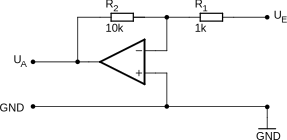
\includegraphics[width=.9\linewidth]{./img/schem-inv.pdf}
		\caption{Basic Inverting Amplifier with Gain 10}
		\label{schem:inv}
	\end{subfigure}
	\begin{subfigure}{0.4\textwidth}
		\centering
		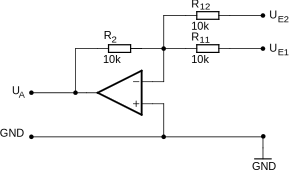
\includegraphics[width=.9\linewidth]{./img/schem-add.pdf}
		\caption{Inverting Adder}
		\label{schem:add}
	\end{subfigure}
	\caption{}
\end{figure}

In the inverting configuration shown in \autoref{schem:inv}, the input signal is fed into the feedback loop, the non-inverting input is held at a fixed voltage.
As the opamp is configured for negative feedback, both inputs are held at the same potential which is often ground.
As the inverting input is not directly connected to a voltage source, it's node is called a 'virtual ground'.

Unlike the non-inverting amplifier, the input of the inverting amplifier has a low input impedance, set by \comp{R_1}.

The gain of the circuit is calculated from the current through \comp{R_1} to the virtual ground node: $I_\comp{R_1} = \frac{\ue}{R_1}$, which is equal to the current through \comp{R_2}: $I_\comp{R_2} = \frac{\ua}{R_2}$.
Using a consistent reference direction, the gain  $A$ is \[A = \frac{\ua}{\ue} = -\frac{R_2}{R_1}.\]

\section{Inverting Adder}

Ignoring \comp{R_1} in \autoref{schem:inv}, the output voltage \ua is $\ua = -R_2 \cdot I_\text{in}$, with the total current $I_\text{in}$ flowing into the virtual ground node of the inverting input.
As the voltage at this node is independent of $I_\text{in}$, more inputs can be connected, each via a resistor that controls the gain of the respective input.
The individual input currents add up to $I_\text{in}$ and the output voltage is \[\ua = -R_2 \cdot \left(\frac{{\ue}_1}{R_{11}} + \frac{{\ue}_2}{R_{12}} + \dots\right),\] with the component labels shown in \autoref{schem:add}.

To test the adder, a sinusoid and a square wave of lower amplitude and higher frequency are fed to the inputs.
The resulting output waveform is shown in \autoref{ss:adder}.

\begin{figure}
	\centering
	\includegraphics[width=.4\linewidth]{./img/ss-adder}
	\caption{Output Waveform Adder}
	\label{ss:adder}
\end{figure}

\section{Inverting Integrator}

\begin{figure}
	\centering
	\begin{subfigure}{0.4\textwidth}
		\centering
		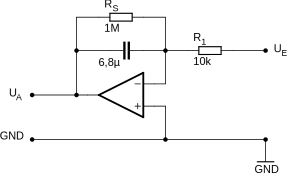
\includegraphics[width=.9\linewidth]{./img/schem-int.pdf}
		\caption{Inverting Integrator}
		\label{schem:int}
	\end{subfigure}
	\begin{subfigure}{0.4\textwidth}
		\centering
		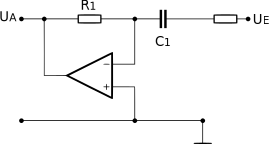
\includegraphics[width=.9\linewidth]{./img/schem-diff.pdf}
		\caption{Inverting Differentiator}
		\label{schem:diff}
	\end{subfigure}
	\caption{}
\end{figure}

Replacing the feedback resistor \comp{R_2} with a capacitor \comp{C_f}, the current through the feedback loop becomes $I_\text{fb} = C_2 \cdot \frac{\diff \ua}{\diff t}$, giving the output voltage \[\ua = - \int \frac{\ue}{C_2 R_1} \diff t + {\ua}_{,0}.\]

The additional 'bleeder' resistor \comp{R_S} slowly discharges \comp{C_f}, eliminating a charge build-up due to a slightly offset input signal and imperfections of components.

\autoref{ss:int} shows the input and output waveforms for square and triangle inputs.

\begin{figure}
	\centering
	\begin{subfigure}{0.4\textwidth}
		\centering
		\includegraphics[width=.9\linewidth]{./img/ss-int-1.jpg}
		\caption{Square Wave Input Signal}
	\end{subfigure}
	\begin{subfigure}{0.4\textwidth}
		\centering
		\includegraphics[width=.9\linewidth]{./img/ss-int-2.jpg}
		\caption{Triangle Wave Input Signal}
	\end{subfigure}
	\caption{Integrator Input (CH1) and Output (CH2)}
	\label{ss:int}
\end{figure}

\section{Inverting Differentiator}

Swapping \comp{R_1} and \comp{C_f} and using the same equations, \ua becomes \[\ua = - R_1 C_1 \frac{\diff \ue}{\diff t}.\]
\autoref{ss:diff} shows the input and output waveforms for square and triangle inputs.

\begin{figure}
	\centering
	\begin{subfigure}{0.4\textwidth}
		\centering
		\includegraphics[width=.9\linewidth]{./img/ss-diff-1.jpg}
		\caption{Square Wave Input Signal}
	\end{subfigure}
	\begin{subfigure}{0.4\textwidth}
		\centering
		\includegraphics[width=.9\linewidth]{./img/ss-diff-2.jpg}
		\caption{Triangle Wave Input Signal}
	\end{subfigure}
	\caption{Differentiator Input (CH1) and Output (CH2)}
	\label{ss:diff}
\end{figure}
